% !TeX root = ../main.tex
\chapter{视觉里程计}
视觉SLAM主要分为视觉前端和后端优化。前端也称为视觉里程计,这是通过相邻图像间的信息估计出粗略的相机运动,给后端提供较好的初始值。视觉里程计的实现也分几种,按照是否需要提取特征,分为特征点法的前端和不提取特征点的直接法前端。基于特征点法的前端被认为是较好的方法,它运行稳定,对光照、动态物体不敏感,是目前比较成熟的解决方案。通过前几章的技术积累,我们已经初步具备了设计一个视觉里程计的能力。\par
\section{单目SLAM的初始化}
对于单目SLAM来说,存在一个尺度问题。我们知道对极几何满足这样的关系:
\begin{equation}
\hat{\boldsymbol{x}}_2^T\left[\boldsymbol{t}\right]_{\times}\boldsymbol{R}\hat{\boldsymbol{x}}_1=0
\end{equation}
可以看到,在方程两边同时乘以某个常数,方程仍然成立。这就意味着从本质矩阵E估计出的t是不可靠的。所以我们并不能连续计算两幅相邻的图片去估计相机的位姿。那解决这个问题的方法就是对前两幅图片的$\boldsymbol{t}$进行归一化,后续的图片通过PnP(后面会介绍)来计算R和t。在单目视觉中,我们对初始两张图像的$\boldsymbol{t}$归一化相当于固定了尺度。虽然我们并不知道$\boldsymbol{t}$的单位是多少,但是我们可以以前两幅图的移动为单位1,以此计算特征点的3D位置。由以上描述我们也可以知道,前两幅图的位置关系不能是纯旋转。纯旋转的两张图无法进行初始化。
\section{三角测量}
\begin{figure}[H]
	\centering
	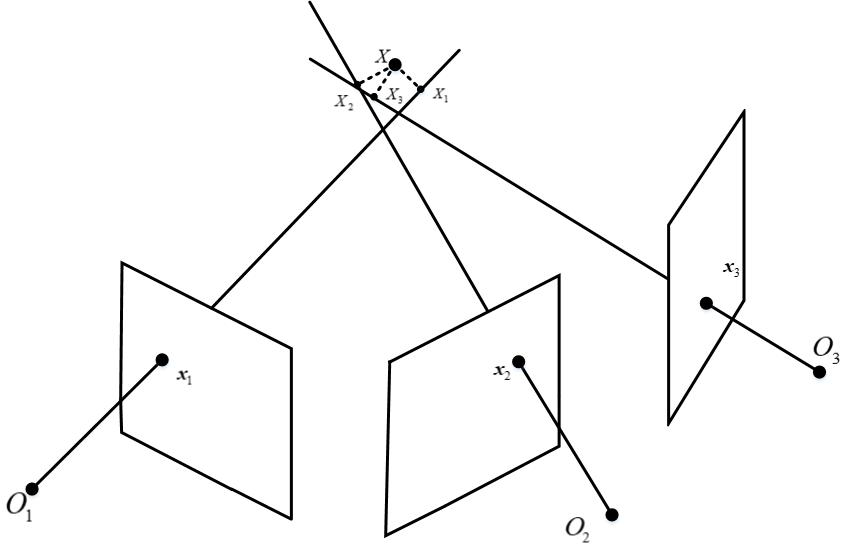
\includegraphics[height=5cm]{triangulation}
	\caption{三角化}
	\label{fig:triangulation}
\end{figure}
假如我们设$x_1,x_2$为两个特征点的归一化坐标,那么他们满足:
\begin{equation}
	s_1\boldsymbol{x_1}=s_2\boldsymbol{Rx_2}+\boldsymbol{t}
\end{equation}
现在我们已经解得$\boldsymbol{R},\boldsymbol{t}$,想要求解出$s_1,s_2$。以求解$s_2$为例,先在两边叉乘一个$x_1$:
\begin{equation}
s_1\left[\boldsymbol{x_1}\right]_{\times}\boldsymbol{x_1}=0=s_2\left[\boldsymbol{x_1}\right]_{\times}\boldsymbol{Rx_2}+\left[\boldsymbol{x_1}\right]_{\times}\boldsymbol{t}
\end{equation}
式子左侧为0,右边的R和t以及$x_1,x_2$都是已知的,由此求得$s_2$。OpenCV中提供了cv::triangulatePoints()函数来实现三角测量。
\section{PnP方法}
上面提到,在求解后面的图片的时候,并不会用到分解本质矩阵得到$R,t$的方法来定位,而是采用PnP(Perspective-n-Point)求解。PnP是求解3D到2D点对的方法。当我们知道n个3D空间点的位置及其投影位置时,如何估计相机位姿。如果两张图像中的一张特征点3D位置已知,那么至少需要3个点对就可以估计相机运动。这种3D-2D方法不需要用到对极约束,又可以在很少的匹配点中获得较好的运动估计,是一种最重要的姿态估计方法。\par
PnP的求解方法有很多种,P3P\cite{gao2003complete}、直接线性变换(DLT)、EPnP\cite{lepetit2009epnp}、UPnP\cite{penate2013exhaustive}等。也可以用非线性优化的方式求解,也就是Bundle Adjustment。
\subsection{直接线性变换}
考虑某个空间点P,它的齐次坐标为P={}
\subsection{非线性优化}





